\documentclass[14pt,dvipsnames]{extarticle}

\usepackage[T1]{fontenc}

\usepackage{microtype}
\DisableLigatures{encoding=*,family=razor}

\usepackage{url}
\usepackage{calc}
\usepackage{xspace}
\usepackage{parskip}

\usepackage[pdftex]{graphicx}
\usepackage{pdfpages}

\usepackage{multicol}
\newenvironment{columns}
{\begin{multicols}{2}
%\@afterindentfalse%\@afterheading
}
{\end{multicols}
\ignorespacesafterend
}

\usepackage[dvipsnames]{colortbl}

\newcommand{\cfbox}[2]{%
    \colorlet{currentcolor}{.}%
    {\color{#1}%
    \fbox{\color{currentcolor}#2}}%
}

\def\twodigits#1{\ifnum#1<10 0\fi\the#1}

%%----------------------------------------------------------------------
%%-- Notes

\usepackage[many]{tcolorbox}

\newtcolorbox{recon}[1][]{
  colback=RedOrange!16,
  colframe=RedOrange,
  fonttitle=\bfseries,
  /tcb/fontupper=\it,
%  title=RECON+,
  #1}

%%----------------------------------------------------------------------
%%-- Font

\usepackage[scaled]{helvet}
\renewcommand*\familydefault{\sfdefault}

%%----------------------------------------------------------------------
%%-- Geometry

\usepackage[letterpaper, portrait, margin=0.5in, bottom=0.5in, footskip=0.25in]{geometry}

\setlength{\columnsep}{0.35in}

%\raggedcolumns

%%----------------------------------------------------------------------
%%-- Headers & Footers

%%----------------------------------------------------------------------
%%-- Sections

\usepackage{titlesec}
%\newcommand{\sectionbreak}{\clearpage}

%\titleformat{\section}[hang]
%  {\usefont{T1}{qhv}{b}{n}}
%  {}
%  {0em}
%  {\hspace{-0.4pt}\Large \thesection\hspace{0.6em}}

\titleformat{name=\section,numberless}[block]
  {\Large\usefont{T1}{razor}{m}{n}} %
  {}
  {0pt}
  {\colorsection}

\newcommand{\pagetitle}[1]{%
  \clearpage
  \fancyfoot[L]{\footnotesize\usefont{T1}{razor}{m}{n}[~#1~]}
  \section{#1}
}

\newcommand{\colorsection}[1]{%
  \colorbox{CornflowerBlue}{\parbox{\dimexpr\textwidth-2\fboxsep}{\hspace{.375\baselineskip}\textcolor{White}{#1}\vspace{.25\baselineskip}}}}

\titleformat{name=\subsection,numberless}[block]
  {\large\usefont{T1}{razor}{m}{n}} %
  {}
  {0pt}
  {\colorsubsection}

\newcommand{\colorsubsection}[1]{%
  \colorbox{CornflowerBlue!10}{\parbox{\dimexpr\textwidth-2\fboxsep}{\hspace{.375\baselineskip}\textcolor{CornflowerBlue}{#1}\vspace{.25\baselineskip}}}}

\titlespacing*{\section}
{0pt}% left margin
{16pt}% before
{8pt}% after

\titlespacing*{\subsection}
{0pt}% left margin
{16pt}% before
{4pt}% after

\newcommand{\missionrule}[1]{\noindent\textbf{#1}\xspace}

%%----------------------------------------------------------------------
%%-- Lists

\newenvironment{squishitemize}
{\begin{list}{$\bullet$}{%
    \setlength{\itemsep}{2pt}%
    \setlength{\parsep}{2pt}%
    \setlength{\topsep}{2pt}%
    \setlength{\parskip}{0pt} %
%    \setlength{\labelwidth}{.5in}%
%    \setlength{\labelsep}{0.05in} %
%    \setlength{\leftmargin}{0.2in} %
    \renewcommand{\labelitemi}{--}}}
  {\end{list}}

%%----------------------------------------------------------------------
%%-- Paragraphs

\setlength{\parskip}{0.8\baselineskip}%

\newcommand{\reconplus}{\textbf{RECON+}\xspace}

\setcounter{secnumdepth}{0}

\usepackage[dotinlabels]{titletoc}

\titlecontents{section}[7mm]% [left]
    {\addvspace{-2pt}}% {above}
    {\bf\contentslabel{7mm}}% {before with label}
    {}% {before without label}
    {\bf\titlerule*[2.7mm]{.}\contentspage}% {filler and page}
    [\addvspace{0mm}]% [after]

\titlecontents{subsection} [17mm]
    {}
    {\contentslabel{10mm}}
    {}
    {\titlerule*[2.7mm]{.}\contentspage}

\titlecontents{subsubsection} [30mm]
    {}
    {\contentslabel{13mm}}
    {}
    {\titlerule*[2.7mm]{.}\contentspage}

\setcounter{tocdepth}{1}


\usepackage{multicol}
\usepackage{multirow}
\usepackage{amsmath}
\usepackage{tabularx}
\usepackage{array}
\newcolumntype{C}[1]{>{\centering\let\newline\\\arraybackslash\hspace{0pt}}m{#1}}
\newcolumntype{F}[1]{>{\centering\let\newline\\\arraybackslash\hspace{0pt}}p{#1}}
\newcolumntype{L}[1]{>{\raggedright\let\newline\\\arraybackslash\hspace{0pt}}m{#1}}
\newcolumntype{R}[1]{>{\raggedleft\let\newline\\\arraybackslash\hspace{0pt}}m{#1}}
\newcolumntype{E}[1]{>{\raggedright\let\newline\\\arraybackslash\hspace{0pt}}p{#1}}
\newcolumntype{R}[1]{>{\raggedleft\let\newline\\\arraybackslash\hspace{0pt}}m{#1}}
\newcolumntype{O}[1]{>{\raggedleft\let\newline\\\arraybackslash\hspace{0pt}}p{#1}}

\usepackage{latexsym}

\usepackage{fancyhdr}
\fancypagestyle{plain}{%
\fancyhf{}
\fancyfoot[C]{\footnotesize\usefont{T1}{razor}{m}{n}[~\thepage~]}
\fancyfoot[R]{\footnotesize\usefont{T1}{razor}{m}{n}[~RECON+~]}
\renewcommand{\headrulewidth}{0pt}
\renewcommand{\footrulewidth}{0pt}}
\pagestyle{plain}


\usepackage{eso-pic}

\newcommand\BackgroundPic[1]{%
\put(0,0){%
\parbox[b][\paperheight]{\paperwidth}{%
\vfill%
\centering%
\includegraphics[width=\paperwidth,height=\paperheight,keepaspectratio]{#1}%
\vfill%
}}}

\newcommand{\squelchbackground}{%
\ClearShipoutPicture
}

\newcommand{\restorebackground}{%
\setbackground
}
\newcommand{\setbackground}{%
\AddToShipoutPicture{\BackgroundPic{art/background/background.pdf}}%
}

%%----------------------------------------------------------------------
%%----------------------------------------------------------------------
\begin{document}
\thispagestyle{empty}
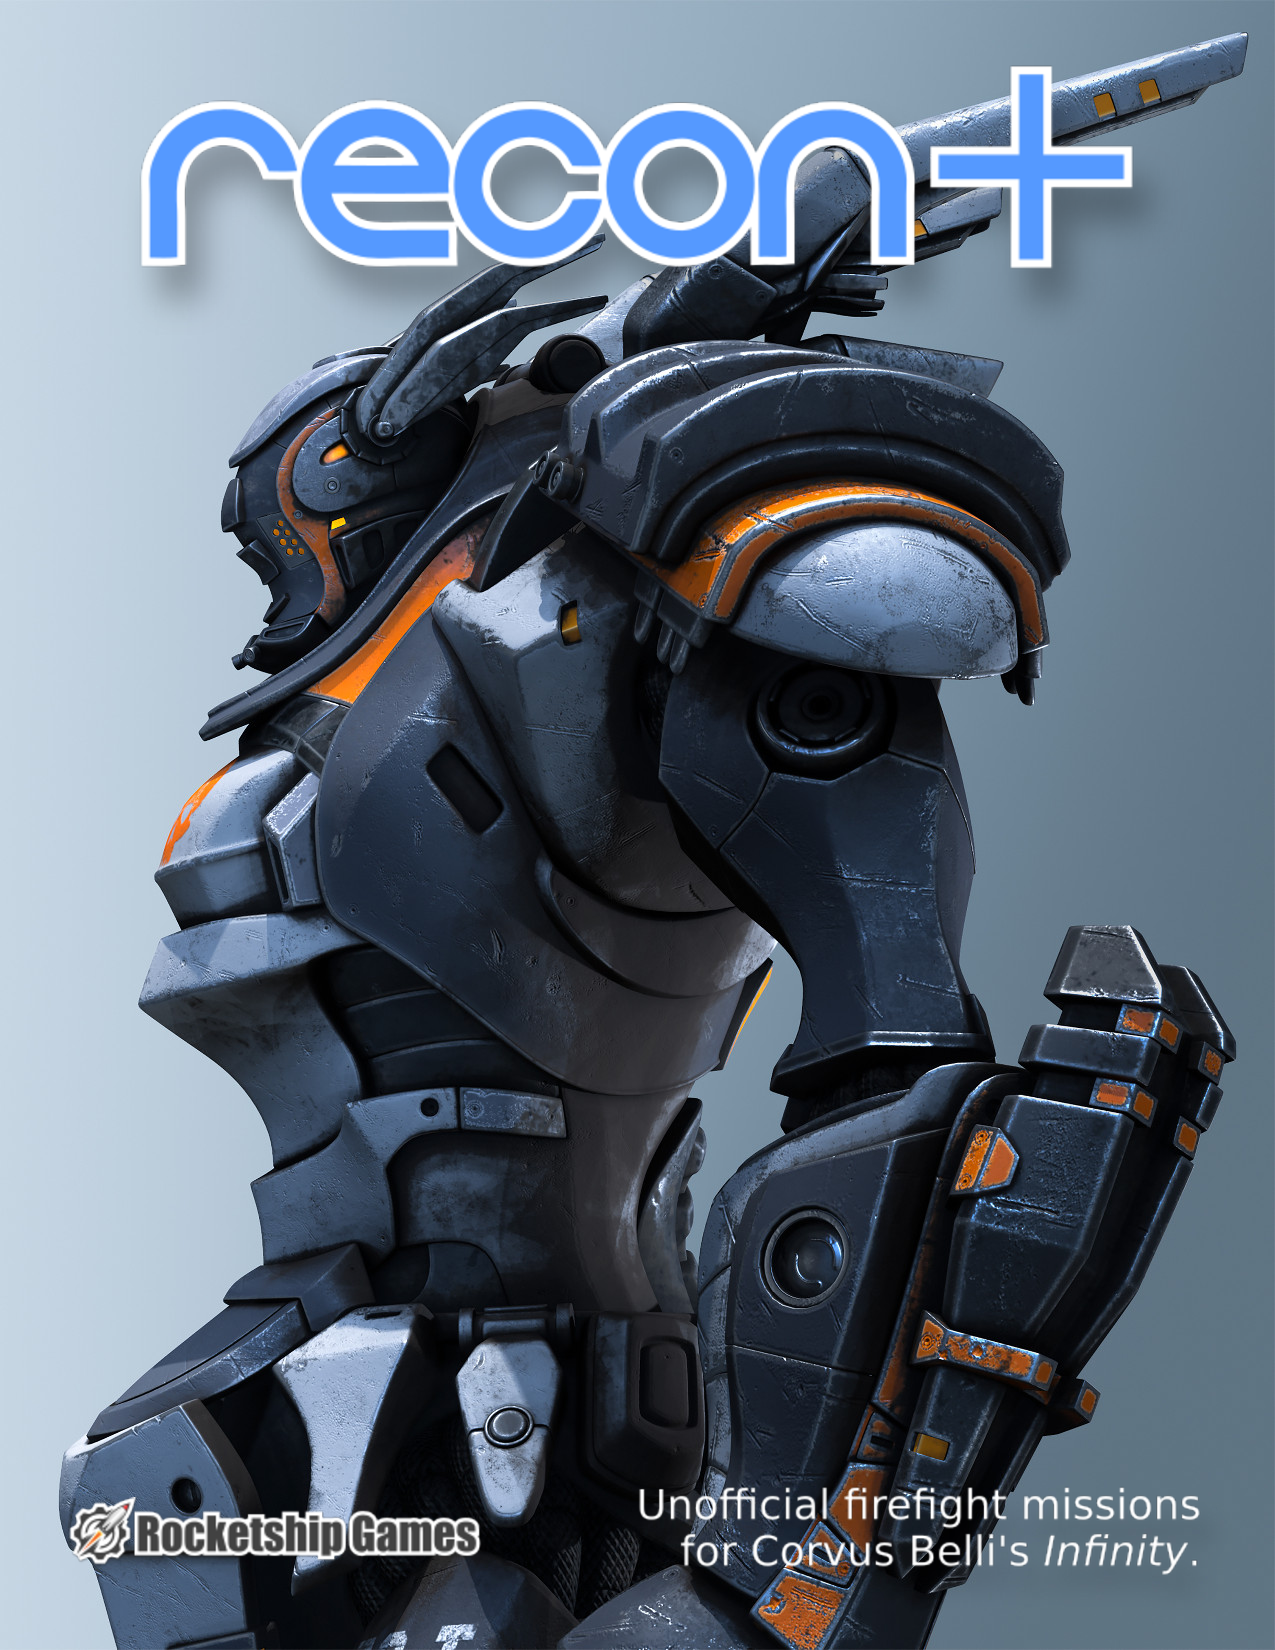
\includepdf[pages={1}]{art/cover/cover.pdf}

\clearpage

%\setbackground
%\setcounter{page}{1}
\fancyfoot[L]{\footnotesize\usefont{T1}{razor}{m}{n}[~Introduction~]}

\begin{figure*}[t!]
  \centering
  
\includegraphics{art/cover/title.pdf}
\end{figure*}

\reconplus is a set of unofficial firefight missions for Corvus
Belli's \emph{Infinity} miniatures game.  Armies are small, the action
fast, games quick, and atypical tactics and strategies required.

Though it works as a stepping stone, \reconplus is not primarily
designed to be an introductory or teaching mode.  It's simply a
different way to play.  All the \emph{Infinity} rules apply and the
missions are strategically deep, but the small armies and play areas
combined with a few gameplay tweaks emphasize different units,
weapons, and tactics.  A line trooper with a combi-rifle should never
be discounted in \emph{Infinity}, but \reconplus is their time to
shine.

%\emph{Get in there, soldier!}

Changes to \reconplus for the \emph{N5} edition of \emph{Infinity}
include:
\begin{squishitemize}
\item Squad construction limitations have been removed as order
  generation and other aspects are now much better balanced across
  troop types than in earlier editions.

\item The restriction to a single fireteam has been removed as the
  benefits of fireteams are not as strong as previous and they are now
  available to the core factions.

\item Troopers no longer need to be Specialist Troops to activate
  objectives, but specialists provide enhanced reliability, making
  squads less fragile in button-pushing missions.

  % and enables using a single list across more mission classes.

%\item Alternate match list selection formats are suggested for
%  organized play.
\end{squishitemize}

\tableofcontents

\vspace{-16pt}
\hbox to 0pt{}\hfill{\small \emph{N5} edition; updated \the\year/\twodigits\month/\twodigits\day}

\clearpage
\fancyfoot[L]{\footnotesize\usefont{T1}{razor}{m}{n}[~Squad Construction~]}

\section{Squad Construction}

\reconplus army lists are chosen according to the following rules:

\vspace{-0.5em}
\begin{itemize}
\item Army lists may include at most~150 army points and~3 SWC.

\item The entire army list must be organized within a single combat
  group.

%\item Troopers with classification Character are not permitted.
%
%\item Only one trooper with the Impetuous, Tactical Awareness, or
%  Strategos skills may be included per every~4 troopers.  The Frenzy
%  skill is not limited.
%
%\item Only one trooper with multiple wounds, structure, or profiles
%  (e.g., Symbiont Armor), or the No Wound Incapacitation skill, may be
%  included per every~4 troopers.

\end{itemize}

All other army list selection rules from the core rules apply, e.g.,
requiring a Lieutenant.

%\begin{recon}
%Note that, as elaborated in the gameplay rules, in \reconplus a player
%may only have a single fireteam of any type active at any time, with a
%maximum of~3 members.
%\end{recon}

\subsection{Army List Selection}

Most \emph{Infinity} organized play has players bring two army lists
from which they choose one each round after their mission, opponent,
and play area (table) are determined.  For both casual and organized
\reconplus play, it's worth considering two other options:
\begin{squishitemize}
  \item \emph{Tailored:} Army lists are composed after establishing
    mission, opponent, and play area. In a tournament, players would
    be given time to construct lists at the start of each match,
    utilizing the same faction throughout but otherwise not
    necessarily related.

  \item \emph{Generalist:} Army lists are composed before knowing any
    match details and are used across multiple missions. In a
    tournament, players would bring a single army list that they have
    to make work in each game.  Missions might not even be determined
    until the start of the event or rounds.  This permits a very fast
    paced event schedule and encourages all-purposes lists and units
    able to achieve varied mission objectives.

\end{squishitemize}

%\subsection{Extras}
%
%Players or event organizers may optionally permit either or both of
%the following extras:
%
%\begin{itemize}
%\item \emph{Spec-Ops:} Army lists may include a single Spec-Ops trooper of up to~12~XP.
%
%\item \emph{Soldiers of Fortune:} Army lists may include up to~38 army
%  points of Mercenary Troops, respecting their AVA, or a single
%  Mercenary Troop selection of any army point value (e.g., a single
%  mercenary TAG may be included by itself despite the~38pt limit).
%\end{itemize}
%
%All other standard \emph{Infinity N4} rules, addendums, and FAQs apply.


\fancyfoot[L]{\footnotesize\usefont{T1}{razor}{m}{n}[~Rules~]}
\section{Play Area}

\reconplus games take place in a play area~22--28in wide and~30--36in
long.  In typical missions with deployment zones along the opposed
short edges, the depth of the deployment zones should be calculated
such that they are 24in apart, i.e.:

\bigskip
\centerline{%
\begin{tabular}{C{1in}C{2in}}
  \rowcolor{CornflowerBlue}\textcolor{White}{\textbf{Play Area Length}} & \textcolor{White}{\textbf{Deployment Zone Depth}} \\
  30in & 3in\\
  \rowcolor{CornflowerBlue!10} 32in & 4in\\
  34in & 5in\\
  \rowcolor{CornflowerBlue!10} 36in & 6in
\end{tabular}
}

%Be sure to place terrain to minimize long firelanes.  At least one
%piece of terrain should touch each play area edge to prevent open
%spaces running its full length.  The tallest terrain should be toward
%the middle of the play area, to prevent creating a ``sniper bowl.''

\begin{recon}
  The mats in Corvus Belli's recent \emph{Infinity} starter terrain
  sets are 24in by 34in.  Some older \emph{Infinity} starter sets had
  mats 32in long.  Mats and boards for Games Workshop's widely played
  \emph{Kill Team} are 22in by 30in.  Organizers should not
  necessarily feel that all tables within an event need to use exactly
  the same play area dimensions.
\end{recon}


\section{Gameplay}

The following rules apply in all \reconplus games unless excepted by a
mission or event.

%\subsection{Pregame}
%
%Match preparation proceeds as follows.
%
%\missionrule{Startup Sequence.}  The following sequence is used in
%setting up each match---
%
%\begin{squishitemize}
%\item Establish mission, opponents \& factions, and play area.
%
%%\item Select classified objectives (see below).
%
%\item Determine army lists as permitted (by selection or composition).
%
%\item Initiative Roll.
%
%\item Deployment Phase.
%
%\item Simultaneously reveal chosen army lists (the public information).
%\end{squishitemize}
%

%\missionrule{Classified Objectives.}  Before choosing their army list,
%each player draws~2 classified objective cards and secretly chooses~1
%to keep in play for themselves (do not reveal either).  Achieving
%classified objectives, including the Secure HVT option (see below), is
%worth~2 objective points in each \reconplus mission.  They may only be
%scored once.

%\missionrule{High Value Targets.}  Each player must deploy a High
%Value Target~(HVT) model at the beginning of their deployment.  These
%must be placed at least~4'' outside of both deployment zones, directly
%on the play area itself (not on any terrain).  A player may opt at any
%point to replace their chosen classified objective with the Secure HVT
%classified objective:

%\begin{squishitemize}
%\item \textbf{Secure HVT} is accomplished if at game end you have a
%  trooper not in a Null state inside the zone of control of the enemy
%  HVT model, and at the same time there are no enemy troopers not in a
%  Null state within the zone of control of your own HVT model.
%\end{squishitemize}

\subsection{Strategic Use of Command Tokens}

The Command Token: Strategic Use options are unaltered caveat the
following.

\missionrule{Order Denial.} The second player may make Strategic Use
of a Command Token to remove a single Regular Order from their
opponent's order pool in the latter's first player turn if their
opponent generated ten orders or less (including Regular, Irregular,
and Tactical Orders).  If more than ten orders were generated they may
remove two Regular Orders.

\missionrule{Logistical.} Whether Speedball Tokens may be used should
be decided before list selection.


\subsection{In-Game}

The following in-game rules apply to all \reconplus matches.

%\missionrule{Limited Fireteams.}  A player may only have a single
%fireteam active at any point in time, across all types.  That fireteam
%may be comprised of a maximum of~3 members.  Forming a fireteam
%automatically and immediately dissolves a player's existing fireteam.

\missionrule{Exclusion Zone.}  Troopers may not be deployed into
Exclusion Zones, as specified by some missions, by any means in either
deployment or gameplay.  This includes Combat Jump, Infiltration, and
all other skills.  Deployable Weapons are not subject to this
constraint.

\missionrule{Specialist Troops.}  Hackers, Doctors, Engineers, Forward
Observers, Paramedics, and troopers with Chain of Command or
Specialist Operative are considered Specialist Troops.  Peripheral
(Servant) models cannot perform tasks reserved for Specialist Troops.

\missionrule{Connect Mission Objective.} Some missions make the
following short skill available.
\label{sec:hack-objective}

\medskip\centerline{\setlength\fboxrule{2pt}
\cfbox{LimeGreen}{\begin{minipage}{6.5in}
  \colorbox{LimeGreen}{\parbox{\linewidth-2\fboxsep}{\textcolor{White}{\textbf{\large Connect Mission Objective} \hfill Short Skill}}}\\
  \colorbox{SkyBlue}{\parbox{\linewidth-2\fboxsep}{\textcolor{White}{Attack}}}

  \medskip
  \textsc{Requirements}
  \begin{squishitemize}
  \item The user must be a model (not a marker) in base contact with a
    mission objective marker or terrain piece.
  \end{squishitemize}

  \medskip
  \colorbox{Gray!24}{\begin{minipage}{\linewidth-2\fboxsep}

  \medskip
      \textsc{Effects}
      \begin{squishitemize}
      \item The user makes a Normal WIP roll to attempt connecting to
        the mission objective marker or terrain piece with which it is
        in base contact.  Specialist Troops roll~+1B and one die of
        their player's choice is discarded.

      \item If successful, the user's player is connected to the
        mission objective; mark it appropriately.  The other player is
        no longer connected to this mission objective if they
        previously were; remove any such marking.
      \end{squishitemize}
    \end{minipage}}
\end{minipage}}}


\subsection{Endgame}

The following outline endgame and scoring conditions for \reconplus
missions.

\missionrule{Game End.}  All matches conclude at the end of the third
game round.  Unless noted otherwise by a mission or event,
\emph{Retreat!} rules do not apply.  If one player is eliminated the
surviving player may play out their remaining turns attempting to
score objectives.

\begin{recon}
  For beginner and casual events a 90 minute round time limit is
  recommended. Experienced players can typically complete RECON+ games
  in about 60 minutes.
\end{recon}

\missionrule{Scoring.}  All standard \reconplus missions are scored out of a
possible~7 objective points.  Players do NOT automatically receive
maximum points for eliminating their opponent.

%\begin{recon}
%  If your opponent cripples your ability to achieve the mission
%  objectives before you eliminate them, then you have not actually
%  earned a full victory!
%\end{recon}

\missionrule{Destroyed.} Troopers are considered destroyed when they
enter the Dead state, are in a Null state at the end of the game, or
have not been deployed by the end of the game.

%Those troopers not
%destroyed are considered to have survived, as are troopers in
%\emph{Retreat!} which exit the play area through the long edge of
%their player's deployment zone.

\missionrule{Domination.}  A player dominates a Sector, as determined
in some missions, if they have more victory points within the Sector
than their opponent.  Only troopers represented by a model or marker,
including Proxies and Peripherals, are counted.  Note that this
excludes troopers in Hidden Deployment.  Troopers are considered to be
solely within the single Sector, if any, containing more than half
their base or marker.  Troopers in a Null state are not counted unless
the state specifically notes otherwise.  For purposes of Domination,
troopers in Shasvastii-Embryo state are counted both during the game
and at game end.

%\clearpage
\section{Mission Elements}

Most \reconplus missions revolve around interacting with elements of
the \emph{Infinity} world as defined in each scenario.  These elements
may be represented by a physical terrain piece or a marker as is
convenient.  If a marker is used they are considered to have the
silhouettes given below and provide cover or block line-of-fire (LOF)
accordingly.

% except Civilians, which do neither.

%\begin{recon}
%  This is a slight variance from the main \emph{Infinity} rulebook, in
%  which mission elements such as objectives only grant cover when
%  physically represented by 3D terrain pieces.
%\end{recon}

Mission elements cannot be directly targeted by attacks or skills
other than those provided by missions.  They are otherwise effectively
terrain, unaffected by indirect attacks, e.g., an Impact Template, and
only affecting attacks as terrain would, such as by providing cover.

\bigskip
\centerline{
\begin{tabular}{cccccc}
  \rowcolor{CornflowerBlue}\textcolor{White}{\textbf{Element}} & \textcolor{White}{\textbf{Type}} & \textcolor{White}{\textbf{ARM}} & \textcolor{White}{\textbf{BTS}} & \textcolor{White}{\textbf{W/STR}} & \textcolor{White}{\textbf{Silhouette}} \\
  Antenna & Scenery Item & 4 & 3 & 2 & S6~ (40mm base x 55mm high)\\
  \rowcolor{CornflowerBlue!10} Console & Scenery Item & 0 & 0 & 1 & S5~ (40mm base x 45mm high)\\
%  Civilian & Neutral Model & 0 & 0 & 1 & S1- (20mm base x 25mm high)\\
%  HVT & Neutral Model & 0 & 0 & 1 & S2~ (25mm base x 40mm high)\\
  Tech-Coffin & Scenery Item & 1 & 0 & 1 & S5~ (40mm base x 45mm high)\\
\end{tabular}
}

%\begin{recon}
%  Civilians have a 20mm base here to denote them as diminutive,
%  cowering, and not cover (by \emph{Human Sphere} they do not block
%  LOF).  Feel free to use 25mm bases/markers.
%\end{recon}

%\vfill
%\centerline{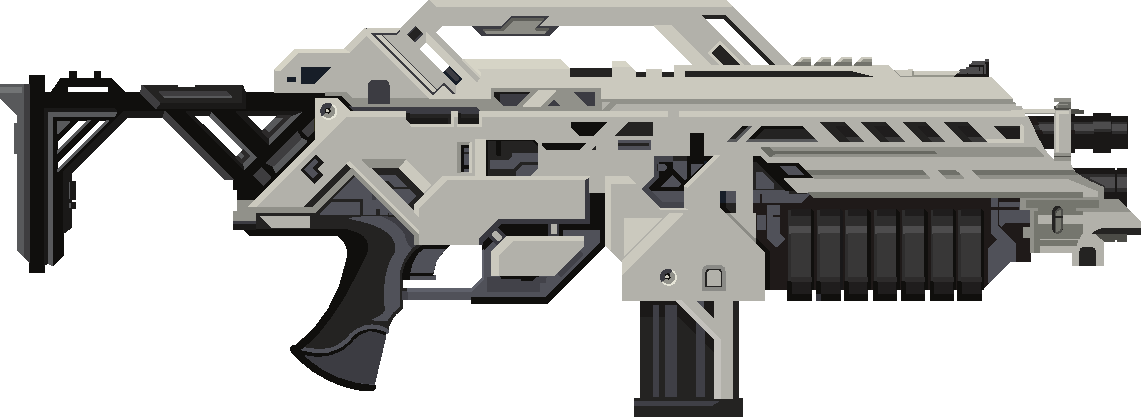
\includegraphics[width=0.6\linewidth]{art/rifle.pdf}}
%\vfill
%\vbox to 0pt{}

%\clearpage
%\fancyfoot[L]{\footnotesize\usefont{T1}{razor}{m}{n}[~\rightmark~]}

%%----------------------------------------------------------------------
\pagetitle{Mission: Annihilate}
\label{mission:annihilation}

\subsection{Play Area Configuration}

There is no special play area configuration for this mission.

\subsection{Mission Rules}

There are no special gameplay rules for this mission.

\subsection{End Game}

There are no special end game conditions for this mission.

\subsection{Scoring}

There are no special scoring rules for this mission.

\noindent%
\begin{tabular}{L{5.85in}C{0.5in}C{0.25in}C{0.25in}}
    \rowcolor{CornflowerBlue} & \textcolor{White}{\textbf{Obj.}} & \multicolumn{2}{c}{\textcolor{White}{\textbf{Player}}}\\
  \rowcolor{CornflowerBlue}\textcolor{White}{\textbf{Condition}} &
                                                                   \textcolor{White}{\textbf{Pts}} & \textcolor{White}{\textbf{1}} & \textcolor{White}{\textbf{2}} \\
  %%
  %% ----------------------------------------------
  At least 25pts of opponent's army list destroyed at game end. & 1 & $\Box$ & $\Box$ \\
  \rowcolor{CornflowerBlue!10} At least 75pts of opponent's army list destroyed at game end. & 1 & $\Box$ & $\Box$ \\
  At least 125pts of opponent's army list destroyed at game end. & 1 & $\Box$ & $\Box$ \\
  \\[-9pt]
%  \rowcolor{CornflowerBlue!10} At least 25pts of player's army list survived at game end. & 1 & $\Box$ & $\Box$ \\
  \rowcolor{CornflowerBlue!10} At least 50pts of player's army list survived at game end.& 1 & $\Box$ & $\Box$ \\
  At least 100pts of player's army list survived at game end. & 1 & $\Box$ & $\Box$ \\
  \\[-9pt]
  \rowcolor{CornflowerBlue!10} More points of opponent's army list destroyed at game end. & 1 & $\Box$ & $\Box$ \\
  \\[-9pt]
  Destroyed at least one of opponent's Lieutenants throughout the game. & 1 & $\Box$ & $\Box$ \\
%  Destroyed more Lieutenants than opponent. & 1 & $\Box$ & $\Box$ \\
  %%
  %% ----------------------------------------------
  \\
\multicolumn{2}{r}{\textbf{Sum:}} & $\rule{0.25in}{0.15mm}$ & $\rule{0.25in}{0.15mm}$\\
\end{tabular}


%%----------------------------------------------------------------------
\pagetitle{Mission: Break Through}
\label{mission:frontline}

\subsection{Play Area Configuration}

There is no special play area configuration for this mission.

\subsection{Mission Rules}

There are no special gameplay rules for this mission.

\subsection{End Game}

\emph{Retreat!} rules DO NOT apply in this mission.

%There are no special end game conditions for this mission.

\subsection{Scoring}

% The following rules determine the outcome of this mission---

\missionrule{Sectors.}  At game end, measure out three Sectors on the
play area each covering the full extent between its long edges:

\begin{squishitemize}
\item One central Sector extending~4'' on both sides of the short
  centerline.
\item Sectors covering the~8'' beyond the central sector toward the
  player edges.
\end{squishitemize}

\begin{recon}
  Note that the deployment zones are purposefully not included in the
  sectors, as that would overly favor the player defending that side
  of the play area.
\end{recon}
%Troops in a null state, other markers (such as deployable equipment),
%fake Holoechoes, and other elements are not counted.

\noindent%
\begin{tabular}{L{5.85in}C{0.5in}C{0.25in}C{0.25in}}
    \rowcolor{CornflowerBlue} & \textcolor{White}{\textbf{Obj.}} & \multicolumn{2}{c}{\textcolor{White}{\textbf{Player}}}\\
  \rowcolor{CornflowerBlue}\textcolor{White}{\textbf{Condition}} &
                                                                   \textcolor{White}{\textbf{Pts}} & \textcolor{White}{\textbf{1}} & \textcolor{White}{\textbf{2}} \\
  %%
  %% ----------------------------------------------
  Dominate the Sector farthest from your deployment zone. & 4 & $\Box$ & $\Box$ \\
  \rowcolor{CornflowerBlue!10} Dominate the Sector at the center of the play area. & 2 & $\Box$ & $\Box$ \\
  Dominate the Sector closest to your deployment zone. & 1 & $\Box$ & $\Box$ \\
  %%
  %% ----------------------------------------------
  \\[-9pt]  
  \rowcolor{CornflowerBlue!10} Classified objective achieved. & 2 & $\Box$ & $\Box$ \\
  \\
\multicolumn{2}{r}{\textbf{Sum:}} & $\rule{0.25in}{0.15mm}$ & $\rule{0.25in}{0.15mm}$\\
\end{tabular}


% %%----------------------------------------------------------------------
\pagetitle{Mission: Exfiltrate}
\label{mission:exfiltrate}

\subsection{Play Area Configuration}

As part of their army deployment, before placing their HVT, each
player deploys~4 Civilian models inside the half of the Exclusion Zone
(see below) on their opponent's side of the play area.  Civilians must
be placed at least~4'' away from all other Civilians.  They cannot be
placed on any terrain requiring a Climb entire order to reach.  No
model or marker may be deployed in base contact with any Civilian or
vice versa.

Once deployed, take~2 Agent and~2 Citizen importance markers (or
suitable proxies indistinguishable on the back side).  Turn them face
down, shuffle them, and randomly assign one to each of your Civilians
without being revealed to you or your opponent.

\missionrule{Exclusion Zone.}  There is an Exclusion Zone
extending~6'' on both sides of the short centerline of the play area
(12'' long total) and covering the full extent between long edges.

\subsection{Mission Rules}

The Interrogate Civilian common skill on the following page is
available in this mission.

Once a Civilian has been revealed as an Agent, it may be directly
targeted by the opposing player as an enemy troop and no penalty is
incurred by them for damaging it.

% The Synchronize Civilian common skill cannot be applied to the
% Civilians in this mission.  Instead the following Common Skill is
% available.

\subsection{End Game}

There are no special end game conditions for this mission.
%(\emph{Retreat!} applies).

\subsection{Scoring}

\missionrule{Exfiltrated.}  An Agent has been Exfiltrated if it is
wholly inside its player's deployment zone.

\missionrule{Secured.}  An Agent is Secured if it is wholly outside
the Exclusion Zone on its player's side of the play area.  An
Exfiltrated Agent is necessarily Secured, but not vice versa.

{\setlength\fboxrule{2pt}
\cfbox{CornflowerBlue}{\begin{minipage}{6.5in}
  \colorbox{CornflowerBlue}{\parbox{\linewidth-2\fboxsep}{\textcolor{White}{\textbf{\large Interrogate Civilian} \hfill Short Movement Skill}}}\\
  \colorbox{SkyBlue}{\parbox{\linewidth-2\fboxsep}{\textcolor{White}{Attack}}}

  \medskip
  \textsc{Requirements}
  \begin{squishitemize}
  \item The user must be a model (not a marker) in base contact with a
    Civilian deployed by their player.

  \item The user cannot already be in CivEvac state with a Civilian,
    unless it possesses the Doctor, Paramedic, or Chain of Command
    special skills, in which case it cannot already be in CivEvac
    state with~2 Civilians.

  \item The user cannot be Impetuous or Extremely Impetuous, including
    through the Frenzy characteristic having triggered.

  \item The user cannot possess the G: Servant or G: Synchronized
    special skills, or its Type of Troop be REM.
    
  \item The user cannot be part of a fireteam of any kind, and this
    short skill cannot be performed as part of a coordinated order.
    
%  \item The targeted Civilian cannot be in the CivEvac state with an
%    enemy model.
  \end{squishitemize}

  \medskip
  \colorbox{Gray!24}{\begin{minipage}{\linewidth-2\fboxsep}

  \medskip      
      \textsc{Effects}
      \begin{squishitemize}
      \item The user makes a Normal WIP roll to synchronize a
        designated Civilian in base contact that was placed by their
        player.  Doctors and Paramedics receive a +3 MOD on this roll.

      \item If the roll is successful, the Civilian's importance
        marker is revealed to both players if it has not already.  If,
        and only if, the Civilian is an Agent, it enters the CivEvac
        state with the user (\emph{Human Sphere}, page~95).

      \item If the roll fails, the opposing player moves the Civilian
        as far as possible following general movement rules up to 2''
        from the user.
      \end{squishitemize}
    \end{minipage}}
\end{minipage}}}

\noindent%
\begin{tabular}{L{5.85in}C{0.5in}C{0.25in}C{0.25in}}
    \rowcolor{CornflowerBlue} & \textcolor{White}{\textbf{Obj.}} & \multicolumn{2}{c}{\textcolor{White}{\textbf{Player}}}\\
  \rowcolor{CornflowerBlue}\textcolor{White}{\textbf{Condition}} &
                                                                   \textcolor{White}{\textbf{Pts}} & \textcolor{White}{\textbf{1}} & \textcolor{White}{\textbf{2}} \\
  %%
  %% ----------------------------------------------
  Have at least one of your Agents in CivEvac state at game end. & 1 & $\Box$ & $\Box$ \\
  \rowcolor{CornflowerBlue!10} Have both of your Agents in CivEvac state at game end. & 1 & $\Box$ & $\Box$ \\
  \\[-9pt]
  Have at least one of your Agents Secured at game end. & 1 & $\Box$ & $\Box$ \\
  \rowcolor{CornflowerBlue!10} Have both of your Agents Secured at game end. & 1 & $\Box$ & $\Box$ \\
  \\[-9pt]  
  Have at least one of your Agents Exfiltrated at game end. & 1 & $\Box$ & $\Box$ \\
  \rowcolor{CornflowerBlue!10} Have both of your Agents Exfiltrated at game end. & 1 & $\Box$ & $\Box$ \\
  \\[-9pt]
  Have more Agents in CivEvac state at game end than your opponent. & 1 & $\Box$ & $\Box$ \\
  %%
  %% ----------------------------------------------
  \\[-9pt]  
  \rowcolor{CornflowerBlue!10} Classified objective achieved. & 2 & $\Box$ & $\Box$ \\
  \\
\multicolumn{2}{r}{\textbf{Sum:}} & $\rule{0.25in}{0.15mm}$ & $\rule{0.25in}{0.15mm}$\\
\end{tabular}

%%----------------------------------------------------------------------
\pagetitle{Mission: Seize the Antennas}
\label{mission:seizetheantennas}

\subsection{Play Area Configuration}

Place one Antenna at the center of the play area and two more
each~10'' from the center on the long centerline toward the deployment
zones (2'' outside the deployment zones).  No model or marker may be
deployed in base contact with an Antenna.

%\begin{recon}
%  In the original RECON packet the outer Antennas are placed 12'' from
%  the center, thus partially within the deployment zones.
%\end{recon}

\subsection{Mission Rules}

The Hack Mission Objective short skill is available in this scenario
(see page~\pageref{sec:hack-objective}).

\subsection{End Game}

There are no special end game conditions for this mission.
%(\emph{Retreat!} applies).

\subsection{Scoring}

The following scoring conditions are evaluated at game end.

\noindent%
\begin{tabular}{L{5.85in}C{0.5in}C{0.25in}C{0.25in}}
    \rowcolor{CornflowerBlue} & \textcolor{White}{\textbf{Obj.}} & \multicolumn{2}{c}{\textcolor{White}{\textbf{Player}}}\\
  \rowcolor{CornflowerBlue}\textcolor{White}{\textbf{Condition}} &
                                                                   \textcolor{White}{\textbf{Pts}} & \textcolor{White}{\textbf{1}} & \textcolor{White}{\textbf{2}} \\
  %%
  %% ----------------------------------------------
  Connected to the Antenna closest to your deployment zone. & 1 & $\Box$ & $\Box$ \\
  \rowcolor{CornflowerBlue!10} Connected to the Antenna at the center of the play area. & 2 & $\Box$ & $\Box$ \\
  Connected to the Antenna farthest from your deployment zone. & 4 & $\Box$ & $\Box$ \\
  %%
  %% ----------------------------------------------
  \\[-9pt]  
  \rowcolor{CornflowerBlue!10} Classified objective achieved. & 2 & $\Box$ & $\Box$ \\
  \\
\multicolumn{2}{r}{\textbf{Sum:}} & $\rule{0.25in}{0.15mm}$ & $\rule{0.25in}{0.15mm}$\\
\end{tabular}


%%----------------------------------------------------------------------
\pagetitle{Mission: Smash and Grab}
\label{mission:smashandgrab}

\subsection{Play Area Configuration}

Place two Tech-Coffins, each equipped with a Datacube, on the short
centerline of the play area and each 5'' from the center toward a
different long edge (10'' apart).

\missionrule{Exclusion Zone.}  There is an Exclusion Zone
extending~6'' on both sides of the short centerline of the play area
(12'' long total) and covering the full extent between long edges.

\subsection{Mission Rules}

%\missionrule{Smash and Grab}
The following short skills and equipment are available in this mission.

\medskip
\centerline{\setlength\fboxrule{2pt}
\cfbox{LimeGreen}{\begin{minipage}{6.5in}
  \colorbox{LimeGreen}{\parbox{\linewidth-2\fboxsep}{\textcolor{White}{\textbf{\large Smash Tech-Coffin} \hfill Short Skill}}}\\
  \colorbox{SkyBlue}{\parbox{\linewidth-2\fboxsep}{\textcolor{White}{Attack}}}

  \medskip
  \textsc{Requirements}
  \begin{squishitemize}
  \item The user must be a Specialist Troop model (not a marker) in
    base contact with a Tech-Coffin equipped with a Datacube.

%  \item The user must not already be equipped with a Datacube, or, if
%    it also possesses Baggage equipment, must not be equipped with two
%    Datacubes.
  \end{squishitemize}

  \medskip
  \colorbox{Gray!24}{\begin{minipage}{\linewidth-2\fboxsep}

  \medskip
      \textsc{Effects}
      \begin{squishitemize}
%      \item Allows the user to make a Normal WIP roll to break the
%        Tech-Coffin's protections and extract the Datacube.  Hackers
%        receive a +3 MOD.

      \item The user makes a Normal WIP roll to extract the Datacube.
      Doctors and Paramedics receive~+3MOD and~+1B on this WIP check.

      \item If passed, the Tech-Coffin unequips a Datacube and
        the user equips it. % (or an additional
        %Datacube if it possesses Baggage and was already equipped with
        %one).

%      \item This skill may be invoked as many times as desired if the
%        user continues to fail.
      \end{squishitemize}
    \end{minipage}}
\end{minipage}}}

\medskip
\centerline{\setlength\fboxrule{2pt}
\cfbox{LimeGreen}{\begin{minipage}{6.5in}
  \colorbox{LimeGreen}{\parbox{\linewidth-2\fboxsep}{\textcolor{White}{\textbf{\large Grab Datacube} \hfill Short Skill}}}\\
  \colorbox{SkyBlue}{\parbox{\linewidth-2\fboxsep}{\textcolor{White}{Attack}}}

  \medskip
  \textsc{Requirements}
  \begin{squishitemize}
  \item The user must be a model (not a marker) in base contact with a
    a Datacube marker or a friendly troop equipped with a Datacube.
    Note that the user does NOT have to be a Specialist Troop to
    execute this skill.

%  \item The user must not already be equipped with a Datacube, or, if
%    it also possesses Baggage equipment, must not be equipped with two
%    Datacubes.
  \end{squishitemize}

  \medskip
  \colorbox{Gray!24}{\begin{minipage}{\linewidth-2\fboxsep}

      \medskip
      \textsc{Effects}
      \begin{squishitemize}
      \item The user designates a Datacube marker or a friendly model
        equipped with a Datacube in base contact from which to grab a
        Datacube.

%      \item The user automatically equips a Datacube (or an additional
%        Datacube if it possesses Baggage and was already equipped with
%        one).

      \item If a friendly troop was designated, it unequips a
        Datacube.  If a Datacube marker was designated, it is removed
        from play.

      \item The user automatically equips the Datacube.
      \end{squishitemize}
  \end{minipage}}
\end{minipage}}}

\centerline{\setlength\fboxrule{2pt}
\cfbox{LimeGreen}{\begin{minipage}{6.5in}
  \colorbox{LimeGreen}{\parbox{\linewidth-2\fboxsep}{\textcolor{White}{\textbf{\large Drop Datacube} \hfill Short Skill, ARO}}}\\
  \colorbox{SkyBlue}{\parbox{\linewidth-2\fboxsep}{\textcolor{White}{Attack}}}

  \medskip
  \textsc{Requirements}
  \begin{squishitemize}
  \item The user must be equipped with a Datacube.
  \end{squishitemize}

  \medskip
  \colorbox{Gray!24}{\begin{minipage}{\linewidth-2\fboxsep}

      \medskip
      \textsc{Effects}
      \begin{squishitemize}
%      \item By spending a short skill or ARO, the user automatically
%        unequips one Datacube.  Its player places a Datacube marker in
%        base contact with the model or at any point in its movement if
%        it made any.
      \item The user automatically unequips one Datacube.  Place a
        Datacube marker in base contact or at any point in the model's
        movement.
      \end{squishitemize}
  \end{minipage}}
\end{minipage}}}

\medskip
\centerline{\setlength\fboxrule{2pt}
\cfbox{Black}{\begin{minipage}{6.5in}
  \colorbox{Black}{\parbox{\linewidth-2\fboxsep}{\textcolor{White}{\textbf{\large Datacube} \hfill Automatic Equipment}}}\\
  \colorbox{White}{\parbox{\linewidth-2\fboxsep}{Obligatory}}

  \medskip
  \textsc{Requirements}
  \begin{squishitemize}
  \item A model cannot ever be equipped with more than one Datacube,
    unless it also possesses Baggage equipment, in which case it may
    equip two.
  \end{squishitemize}

  \medskip
  \colorbox{Gray!24}{\begin{minipage}{\linewidth-2\fboxsep}

      \medskip
      \textsc{Effects}
      \begin{squishitemize}
%      \item No model may ever be equipped with more than one Datacube,
%        unless it also possesses Baggage equipment, in which case it
%        may be equipped with two Datacubes.

      \item Immediately upon the user entering a Null state (e.g.,
        going Unconscious), their model being replaced with a marker
        (e.g., returning to the Camouflaged state), or being removed
        from the game (e.g., becoming Dead), they unequip the Datacube
        and a Datacube marker is placed by their player in base
        contact with the user or its former position.

        %If they possessed multiple Datacubes, a Datacube marker is
        %placed for each.
      \end{squishitemize}
  \end{minipage}}
\end{minipage}}}

\subsection{End Game}

There are no special end game conditions for this mission.
%(\emph{Retreat!} applies).

\subsection{Scoring}

\missionrule{Hold.} Players hold a Datacube whenever any of
their models are equipped with such.

\vspace*{-1pt}

\noindent%
\begin{tabular}{L{5.85in}C{0.5in}C{0.25in}C{0.25in}}
    \rowcolor{CornflowerBlue} & \textcolor{White}{\textbf{Obj.}} & \multicolumn{2}{c}{\textcolor{White}{\textbf{Player}}}\\
  \rowcolor{CornflowerBlue}\textcolor{White}{\textbf{Condition}} &
                                                                   \textcolor{White}{\textbf{Pts}} & \textcolor{White}{\textbf{1}} & \textcolor{White}{\textbf{2}} \\
  %%
  %% ----------------------------------------------
  Hold any Datacube at the end of game round~1. & 1 & $\Box$ & $\Box$ \\
  \rowcolor{CornflowerBlue!10} Hold any Datacube at the end of game round~2. & 1 & $\Box$ & $\Box$ \\
  Hold any Datacube at the end of game round~3. & 3 & $\Box$ & $\Box$ \\
  \\[-9pt]
  \rowcolor{CornflowerBlue!10} Hold any Datacube at any point throughout the game. & 1 & $\Box$ & $\Box$ \\
  \\[-9pt]
  Hold both Datacubes at the end of the game. & 1 & $\Box$ & $\Box$ \\
  %%
  %% ----------------------------------------------
  \\
\multicolumn{2}{r}{\textbf{Sum:}} & $\rule{0.25in}{0.15mm}$ & $\rule{0.25in}{0.15mm}$\\
\end{tabular}


%%----------------------------------------------------------------------
\pagetitle{Mission: Sweep and Clear}
\label{mission:sweepandclear}

\subsection{Play Area Configuration}

Place~2 Consoles, each 12'' from the play area long edges and 6'' from
the center toward the deployment zones.  No model or marker may be
deployed in base contact with a Console.

\subsection{Mission Rules}

The Hack Mission Objective short skill is available in this scenario.

\subsection{End Game}

There are no special end game conditions for this mission.

\subsection{Scoring}

% The following rules determine the outcome of this mission---

\missionrule{Sectors.}  After each game turn measure four
Sectors on the play area dividing the space between the deployment
zones into equal quarters and determine domination of each.

\missionrule{Tapped Sensor Grid.}  For each Console they control and
have a model in base contact, players may designate a Sector after
each game turn in which they are considered to have an additional~20
army points for purposes of domination.  Both players make this
declaration simultaneously.  A Sector may be designated twice by a
player if they control both Consoles.

\noindent%
\begin{tabular}{L{5.85in}C{0.5in}C{0.25in}C{0.25in}}
    \rowcolor{CornflowerBlue} & \textcolor{White}{\textbf{Obj.}} & \multicolumn{2}{c}{\textcolor{White}{\textbf{Player}}}\\
  \rowcolor{CornflowerBlue}\textcolor{White}{\textbf{Condition}} &
                                                                   \textcolor{White}{\textbf{Pts}} & \textcolor{White}{\textbf{1}} & \textcolor{White}{\textbf{2}} \\
  %%
  %% ----------------------------------------------
  Dominate more Sectors following game turn~1. & 1 & $\Box$ & $\Box$ \\
  \rowcolor{CornflowerBlue!10} Dominate more Sectors following game turn~2. & 2 & $\Box$ & $\Box$ \\
  Dominate more Sectors following game turn~3. & 3 & $\Box$ & $\Box$ \\
  \\[-9pt]  
  \rowcolor{CornflowerBlue!10} Control more Consoles at game end. & 1 & $\Box$ & $\Box$ \\
  %%
  %% ----------------------------------------------
  \\[-9pt]  
Classified objective achieved. & 2 & $\Box$ & $\Box$ \\
  \\
\multicolumn{2}{r}{\textbf{Sum:}} & $\rule{0.25in}{0.15mm}$ & $\rule{0.25in}{0.15mm}$\\
\end{tabular}


\pagetitle{Reference Guides}

\subsection{Random Mission Table}
\bigskip
\medskip
\centerline{
\begin{tabular}{C{0.75in}C{1.75in}C{0.5in}C{1.25in}L{2in}}
  \rowcolor{CornflowerBlue}\textcolor{White}{\textbf{D20}} & \textcolor{White}{\textbf{Mission}} & \textcolor{White}{\textbf{Page}} & \textcolor{White}{\textbf{Elements}} & \textcolor{White}{\textbf{Description}}\\
  1--4 & Annihilate & \pageref{mission:annihilation} & - & Kill them all.\\
  \rowcolor{CornflowerBlue!10} 5--8 & Break Through & \pageref{mission:frontline} & - & Puncture the frontline.\\
%  8--10 & Exfiltrate & \pageref{mission:exfiltrate} & 6 Civilians & Extract your agents.\\
  9--12  & Seize the Antennas & \pageref{mission:seizetheantennas} & 3 Antennas & Hack the transmitters.\\
  \rowcolor{CornflowerBlue!10} 13--16 & Smash and Grab & \pageref{mission:smashandgrab} & 2 Tech-Coffins & Steal the bio-data.\\
  17--20 & Sweep and Clear & \pageref{mission:sweepandclear} & 2 Consoles & Search the area.\\
\end{tabular}
}

\medskip
\centerline{\textit{Seize the Antennas or Annihilate are recommended for introductory games.}}

%\vspace{-0.5em}
\subsection{Play Area Configurations}

\hfill
\begin{minipage}{2in}\centering
\colorbox{CornflowerBlue}{\parbox[t][12pt]{\linewidth-2\fboxsep}{\centering\textcolor{White}{\textbf{Annihilate}}}}

\smallskip
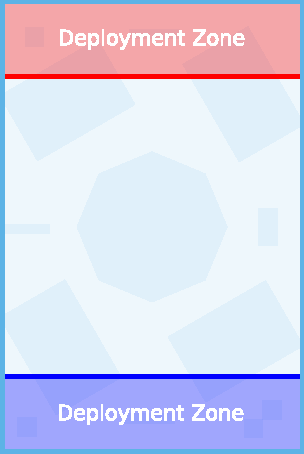
\includegraphics[scale=0.9]{maps/map-annihilate}
\end{minipage}
\hfill
\begin{minipage}{2in}\centering
\colorbox{CornflowerBlue}{\parbox[t][12pt]{\linewidth}{\centering\textcolor{White}{\textbf{Break Through}}}}

\smallskip
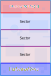
\includegraphics[scale=0.9]{maps/map-breakthrough}
\end{minipage}
\hfill
\begin{minipage}{2in}\centering
\colorbox{CornflowerBlue}{\parbox[t][12pt]{\linewidth}{\centering\textcolor{White}{\textbf{Seize the Antennas}}}}

\smallskip
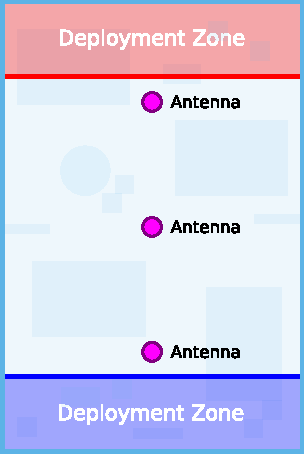
\includegraphics[scale=0.9]{maps/map-seizetheantennas}
\end{minipage}
%\begin{minipage}{2in}\centering
%\colorbox{CornflowerBlue}{\parbox[t][12pt]{\linewidth}{\centering\textcolor{White}{\textbf{Exfiltrate}}}}
%
%\smallskip
%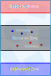
\includegraphics[scale=0.9]{maps/map-exfiltrate}
%\end{minipage}
\hfill
\hbox to 0pt{}

\vspace{-0.5em}
\noindent\hfill
\begin{minipage}{2in}\centering
\colorbox{CornflowerBlue}{\parbox[t][12pt]{\linewidth-2\fboxsep}{\centering\textcolor{White}{\textbf{Smash and Grab}}}}

\smallskip
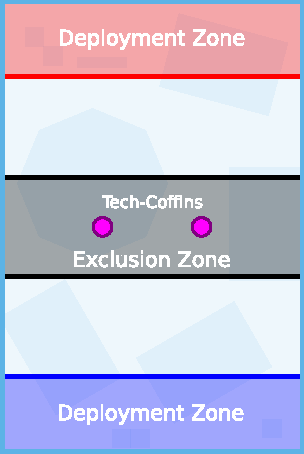
\includegraphics[scale=0.9]{maps/map-smashandgrab}
\end{minipage}
\hfill
\begin{minipage}{2in}\centering
\colorbox{CornflowerBlue}{\parbox[t][12pt]{\linewidth}{\centering\textcolor{White}{\textbf{Sweep and Clear}}}}

\smallskip
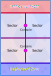
\includegraphics[scale=0.9]{maps/map-sweepandclear}
\end{minipage}
\hfill
\hbox to 0pt{}

\end{document}
